% ************************** Prólogo *****************************
% Use `prologo' as an option in the document class to print only the titlepage and the abstract.

\begin{prologo}\label{prologo}

\subsection*{Prácticas externas}
Este trabajo se ha realizado en el marco del convenio de prácticas de empresa entre la Universidad de Zaragoza y el Laboratorio de Geomática del Instituto Interuniversitario de Geografía de la Universidad de Alicante. El periodo de prácticas ha tenido una duración desde julio hasta noviembre de 2017, sumando un total de 440 horas presenciales.

En el Laboratorio de Geomática se desarrollan actualmente varios proyectos de investigación, entre ellos el Sistema de Información Geográfica de la Universidad de Alicante (SIGUA) es el proyecto de más largo recorrido. SIGUA se puso en marcha en 1997, lo que supone que \textbf{los expertos del laboratorio cuentan con más de 20 años de experiencia en el diseño y gestión de SIG corporativos}. A esta experiencia hay que sumarle numerosos desarrollos de aplicaciones y colaboraciones en otros proyectos de geografía aplicada. Cabe mencionar que el equipo del Laboratorio de Geomática está formado por licenciados, ingenieros y doctores, tanto en Geografía como en Informática, los cuales desarrollan su trabajo en las Tecnologías de la Información Geográfica basadas en \textit{software libre}.

Actualmente, el Laboratorio de Geomática reparte sus esfuerzos entre el mantenimiento e innovación de SIGUA y un proyecto de investigación oficial conocido por su acrónimo como SIOSE-INNOVA: Innovaciones técnicas y metodológicas en el Sistema de Información sobre Ocupación del Suelo de España (SIOSE) y su aplicación en estudios geográficos. Se trata de un proyecto de alcance internacional a través de la \textbf{colaboración con el Instituto Geográfico Nacional (IGN).}

\subsection*{Proyecto SIOSE-INNOVA}
El presente Trabajo Fin de Máster en Tecnologías de la Información Geográfica para la Ordenación del Territorio: SIG y Teledetección, detalla todas las tareas desarrolladas durante la participación en el Proyecto SIOSE-INNOVA. El Investigador Principal de este proyecto es el profesor Alfredo Ramón Morte, quien dirige y coordina una investigación, en la que \textbf{colaboran varias universidades junto con el  Servicio de Ocupación del Suelo del Instituto Geográfico Nacional (IGN), que es el equipo responsable de la base de datos del SIOSE}.

SIOSE-INNOVA es un proyecto de investigación financiado por el Programa Estatal de Investigación, Desarrollo e Innovación Orientada a los Retos de la Sociedad, dentro del Plan Estatal de Investigación Científica y Técnica y de Innovación 2013-2016. Los objetivos principales  de este proyecto tienen \textbf{una parte innovadora}, que consiste en comprobar qué tecnologías \textit{NoSQL} (no sólo SQL) pueden aportar mejores soluciones para la explotación de la base de datos del SIOSE, \textbf{y una parte aplicada}, que consiste en poner en práctica las nuevas tecnologías en casos de estudios reales.

Durante el desarrollo del proyecto SIOSE-INNOVA, se quieren alcanzar los siguientes objetivos específicos:
\begin{enumerate}
\item Crear un marco de experimentación \textbf{\textit{reproducible y fácilmente utilizable}} por un gran número de usuarios.
\item Analizar las necesidades y rendimiento de distintas tecnologías de \textbf{bases de datos NoSQL para la explotación del SIOSE}.
\item Desarrollar e implementar \textbf{un nuevo modelo de datos auxiliar} que permita extender las posibilidades de análisis del SIOSE con técnicas de Big Data o Data Mining.
\item \textbf{Evaluar la \textit{usabilidad} de los datos SIOSE} en distintas plataformas tecnológicas, mediante su aplicación en casos de uso reales en los que utilizar datos de ocupación del suelo resulte esencial.
\end{enumerate}

En la introducción de este trabajo se explica el gran potencial del SIOSE, junto a las dificultades que surgen en bases de datos de ocupación del suelo de estas dimensiones y complejidad. \textbf{El proyecto SIOSE-INNOVA pretende facilitar el uso de la información que contiene el SIOSE.}

Concretamente, este Trabajo Fin de Máster se enmarca dentro del proyecto SIOSE-INNOVA cubriendo la primera etapa del proyecto, en la que se plantea \textbf{una plataforma tecnológica} lo suficientemente potente como \textbf{para analizar el SIOSE de una \textit{manera ágil, intuitiva e interactiva}.}

En este contexto, se ha desarrollado una nueva extensión sobre PostgreSQL/PostGIS, denominada \textbf{\textit{pg\_landmetrics}}, capaz de calcular métricas del paisaje a partir de la base de datos del SIOSE, superando así determinados problemas de \textit{usabilidad} y de escalabilidad (gran volumen de datos). La plataforma de desarrollo descrita en este trabajo (\textit{git, dockers, pgxn, etc}), \textbf{promueve la reproducibilidad} de esta investigación y asegura \textbf{que otros usuarios sean capaces de utilizar lo que aquí se plantea} de una manera lo más sencilla posible, quizás similar a descargar y usar una \textit{app} para teléfonos inteligentes.

El desarrollo del presente trabajo gira entorno a \textbf{un caso de uso} que sirve para valorar la \textit{usabilidad} de todo lo que se desarrollará en el contexto del proyecto SIOSE-INNOVA. Este caso de uso consiste en crear \textbf{un visor de cartografía web} en el que se puedan consultar y analizar los datos del SIOSE. En este trabajo se plantea que dicho visor sirva para \textbf{calcular métricas del paisaje a partir de los datos del SIOSE}. A modo de ejemplo, en la Figura \ref{fig:visorweb} se describe una posible aplicación para calcular las métricas del paisaje de dos zonas geográficas distintas y así comparar su estructura. Cabe adelantar que la experiencia computacional descrita en el Capítulo \ref{chap:result} simula este tipo de aplicación.

Lo deseable en una aplicación como la que descrita (ver Figura \ref{fig:visorweb}) es poder seleccionar una región de España o áreas más pequeñas y \textbf{\textit{consultar el SIOSE de un modo directo}}, sin necesidad de descargar pesados ficheros SIG (ESRI \textit{Shapefile}), unirlos, procesarlos y obtener los resultados tras un proceso relativamente costoso. El tiempo de respuesta de una aplicación similar es muy importante para la experiencia de los usuarios y también para conseguir dar servicio a un gran número de usuarios.

\begin{figure}
\begin{center}
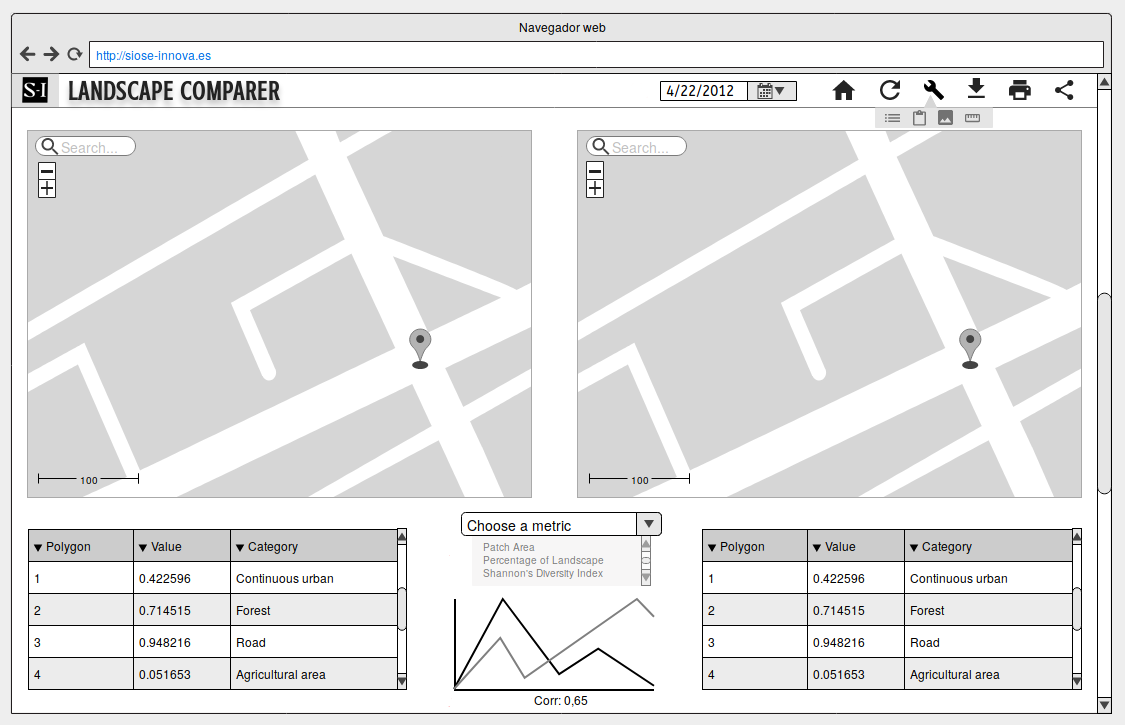
\includegraphics[width=\textwidth]{Prologo/Figs/visorweb.png}
\caption{Prototipo de un visor cartográfico para el análisis (comparación) de la estructura del paisaje a partir del SIOSE. La extensión sobre PostgreSQL/PostGIS desarrollada en este trabajo (\textit{pg\_landmetrics}) es la base para este tipo de aplicaciones. \label{fig:visorweb}}
\end{center}
\end{figure}

La extensión \textit{pg\_landmetrics} encapsula consultas SQL más complejas y \textbf{hace posible calcular múltiples métricas del paisaje en sentencias de una o muy pocas líneas}. Además, esta extensión se instala de un modo sencillo y \textbf{permite trabajar con bases de datos voluminosas} como la del SIOSE (millones de registros; Gigabytes de memoria; ver Tabla \ref{tab:datos}). 

Una cuestión que va más allá de los objetivos de este trabajo tiene que ver con el verdadero potencial de la plataforma de \textit{contenerización} con la que se ha desarrollado \textit{pg\_landmetrics}. Al tratarse de un \textit{software libre} y \textit{contenerizado} (ver capítulo \ref{chap:metod}), se facilita la distribución de esta aplicación a otros equipos (servidores y/o PCs), lo cual \textbf{aporta una escalabilidad que ningún entorno de escritorio puede lograr}. Es decir que a más usuarios del SIOSE, resultaría sencillo añadir nuevos servidores para realizar el análisis.

\subsection*{Estructura del trabajo}
Este trabajo se organiza en cuatro capítulos, a parte las referencias bibliográficas y los anexos. De un modo general, la estructura seguida es la siguiente:
\begin{itemize}
\item En el capítulo \ref{chap:intro} se revisa el uso de las bases de datos de ocupación del suelo y su papel en el análisis de la estructura del paisaje a partir de métricas de paisaje. Al final se presentan los objetivos generales y específicos de este trabajo.

\item En el capítulo \ref{chap:metod} se describen los conjuntos de datos, herramientas, plataformas tecnológicas y metodología seguida para diseñar e implementar una nueva extensión sobre PostgreSQL/PostGIS. La metodología incluye desde el trabajo colaborativo en varias plataformas de desarrollo, hasta las tareas diarias, la incorporación de funciones y la documentación de la extensión. Finalmente, se plantean una serie de experiencias computacionales para evaluar la extensión de acuerdo con los objetivos del trabajo.

\item En el capítulo \ref{chap:result} se detallan todos los resultados obtenidos, tanto en forma de código, como aquellos resultados obtenidos en un caso de estudio que simula una aplicación real (ver Figura \ref{fig:visorweb}).

\item Finalmente, en el capítulo \ref{chap:concl} se revisa el trabajo realizado para valorar cómo se han alcanzado los objetivos propuestos en la introducción. El capítulo termina por detallar los próximos pasos que seguirá el equipo de desarrollo para completar una extensión en \textit{fase de producción} (p. ej. un visor publicado desde una página web del IGN).
\end{itemize}



\end{prologo}
